%; whizzy chapter
% -initex iniptex -latex platex -format platex -bibtex jbibtex -fmt fmt
% 以上 whizzytex を使用する場合の設定。

%     Kansai Debian Meeting resources
%     Copyright (C) 2007 Takaya Yamashita
%     Thank you for Tokyo Debian Meeting resources

%     This program is free software; you can redistribute it and/or modify
%     it under the terms of the GNU General Public License as published by
%     the Free Software Foundation; either version 2 of the License, or
%     (at your option) any later version.

%     This program is distributed in the hope that it will be useful,
%     but WITHOUT ANY WARRANTY; without even the implied warranty of
%     MERCHANTABILITY or FITNESS FOR A PARTICULAR PURPOSE.  See the
%     GNU General Public License for more details.

%     You should have received a copy of the GNU General Public License
%     along with this program; if not, write to the Free Software
%     Foundation, Inc., 51 Franklin St, Fifth Floor, Boston, MA  02110-1301 USA

%  preview (shell-command (concat "evince " (replace-regexp-in-string "tex$" "pdf"(buffer-file-name)) "&"))
% 画像ファイルを処理するためにはebbを利用してboundingboxを作成。
%(shell-command "cd image200708; ebb *.png")

%%ここからヘッダ開始。

\documentclass[mingoth,a4paper]{jsarticle}
\usepackage{kansaimonthlyreport}
\usepackage[dvips]{xy}

% 日付を定義する、毎月変わります。
\newcommand{\debmtgyear}{2012}
\newcommand{\debmtgdate}{26}
\newcommand{\debmtgmonth}{8}
\newcommand{\debmtgnumber}{63}

\begin{document}

\begin{titlepage}

% 毎月変更する部分、本文の末尾も修正することをわすれずに

 第\debmtgnumber{}回 関西 Debian 勉強会資料

\vspace{2cm}

\begin{center}
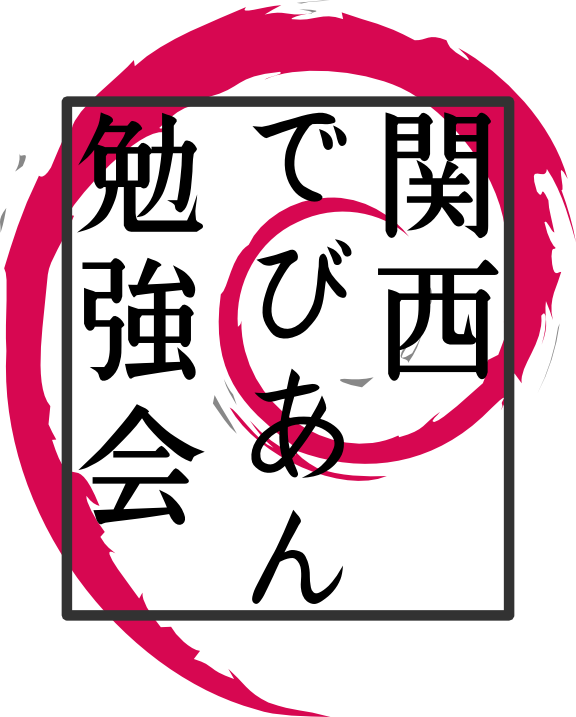
\includegraphics{image200802/kansaidebianlogo.png}
\end{center}

\begin{flushright}
\hfill{}関西 Debian 勉強会担当者 佐々木・倉敷・のがた・かわだ \\
\hfill{}\debmtgyear{}年\debmtgmonth{}月\debmtgdate{}日
\end{flushright}

\thispagestyle{empty}
\end{titlepage}

\dancersection{Introduction}{Debian JP}

 関西Debian勉強会はDebian GNU/Linuxのさまざまなトピック
 (新しいパッケージ、Debian特有の機能の仕組、Debian界隈で起こった出来事、
 などなど)について話し合う会です。

 目的として次の三つを考えています。
 \begin{itemize}
  \item MLや掲示板ではなく、直接顔を合わせる事での情報交換の促進
  \item 定期的に集まれる場所
  \item 資料の作成
 \end{itemize}

 それでは、楽しい一時をお楽しみ下さい。

\newpage

\begin{minipage}[b]{0.2\hsize}
 {\rotatebox{90}{\fontsize{80}{80}
{\gt 関西 Debian 勉強会}}}
\end{minipage}
\begin{minipage}[b]{0.8\hsize}
\hrule
\vspace{2mm}
\hrule
\setcounter{tocdepth}{1}
\tableofcontents
\vspace{2mm}
\hrule
\end{minipage}

\dancersection{最近のDebian関係のイベント報告}{Debian JP}

\subsection{第 62 回関西 Debian 勉強会@OSC012Kansai@Kyoto}

62 回目の関西 Debian 勉強会は今月 3 日、4日に京都リサーチパークで行なわれたオープンソースカンファレンスで行ないました。

セミナーでは「Debian 7.0  ``Wheezy'' frozen」と題して 6 月にフリーズされた次期リリース候補の Debian 7.0 ``Wheezy'' の紹介を行ないました。
ブースの方にも多くの方に立ち寄って頂き、中でも Debian T シャツは大変好評でした。

\subsection{第 91 回東京エリア Debian 勉強会}
91 回目の東京エリア Debian 勉強会は 8 月 2 日に開催されました。

DebConf 12 参加報告、月刊 Debhelper、ソフト開発以外の簡単 Debian contribution(ドラフト版!)、Debian での C++11 開発環境
といった内容でした。

Debian contribution ではソフト開発以外の様々な Debian への貢献方法が紹介されています。
パッケージメンテナンスは難しいけれど何か貢献したいと思われている方は参考にして何かやってみようと思われることから始めてみてはいかがでしょうか。

\dancersection{事前課題}{Debian JP}

今回は以下の課題を出題しました.
\begin{screen}
  \begin{enumerate}
  \item MIT版Kerberosでサービスに必要となるプロセス名と、そのプロセスが使用するポートを 2 つ以上挙げてください。

  \item DebConf12での資料を予習しておいてください。\\
   \url{http://penta.debconf.org/dc12_schedule/events/894.en.html}

  \end{enumerate}
\end{screen}

参加者の皆さんの解答は以下の通りです。

\begin{prework}{ 岡野孝悌 }
  (無回答)
\end{prework}

\begin{prework}{ 川江 }
  \begin{enumerate}
  \item 認証プロセス 749 750
  \end{enumerate}
\end{prework}

\begin{prework}{ とみー }
  \begin{enumerate}
  \item まったくわかりませんが、参加して勉強したいとおもいます。
  \end{enumerate}
\end{prework}

\begin{prework}{ かわだてつたろう }
  \begin{enumerate}
  \item sid 環境で krb5-\{admin-server,kdc\} をインストールして確認。
    \begin{itemize}
    \item krb5kdc 88/udp 750/udp
    \item kadmind 464/udp 464/tcp 749/tcp
    \end{itemize}
  \item 見ておきます。
  \end{enumerate}
\end{prework}

\begin{prework}{ okumura.d }
  \begin{enumerate}
  \item kadmind プロセス。tcp及びudpポート番号は88,749.\\
    \#750(Kerberos RFile)はWindows限定..?
  \end{enumerate}
\end{prework}

\begin{prework}{ 佐々木洋平 }
  \begin{enumerate}
  \item
    \begin{itemize}
    \item process
      \begin{itemize}
      \item krb5-admin-server
      \item krb5-kdc
      \end{itemize}
    \item port
      \begin{itemize}
      \item 88/udp, 754/tcp, 760/tcp
      \end{itemize}
    \end{itemize}
  \item 見ておきまする。
  \end{enumerate}
\end{prework}

\begin{prework}{ 木下 }
  \begin{enumerate}
  \item ケルベロス認証では、「KDC(Key Distribution Center)」と呼ばれるサーバーを用意し、そこに認証情報を一元管理。\\
    →ユーザーが複数サーバーを利用する場合、一度認証を受けるだけで、ほかのサーバーへもアクセスできるようになり、何度もログインする必要がなくなる。
    \begin{enumerate}
    \item サービスに必要となるプロセス名
      \begin{itemize}
      \item krb5kdc(Kerberos サーバー)
      \item kadmin(kadmin ユーティリティ)
      \item krb524(?不明)
      \end{itemize}
    \item サービスに必要となるプロセス名
      \begin{itemize}
      \item すみません。時間がなく調べられていません。
      \end{itemize}
    \end{enumerate}
  \item 時間の許す限り見ておきます。
  \end{enumerate}
\end{prework}

\begin{prework}{ yyatsuo }
  \begin{enumerate}
  \item 勉強しておきます。
  \item 勉強しておきます。
  \end{enumerate}
\end{prework}

\begin{prework}{ 0xBCD1BC92 }
  \begin{enumerate}
  \item インストールしたらわかるのかもしれないが、/etc/init.dのプロセスをキックする名前でお茶を濁しておく。したの/etc/serivcesと連動しているかもしれず。
    \begin{itemize}
    \item krb5-admin-server
    \item krb5-kdc
    \end{itemize}
    /etc/services から拾ったから正解だと思う。
    \begin{itemize}
    \item 88/udp
    \item 754/tcp         krb5\_prop hprop
    \item 760/tcp         kreg
    \end{itemize}
  \item 資料は、仕事の間ににらんでおきます。
  \end{enumerate}
\end{prework}

\begin{prework}{ 西山和広 }
  \begin{enumerate}
  \item kadmind で TCP の 749 と 464
  \end{enumerate}
\end{prework}

\begin{prework}{ 安部武志 }
  \begin{enumerate}
  \item プロセス名: krb5kdc (KDC)\\
    使用するポート番号: 88 および 750
  \end{enumerate}
\end{prework}

\begin{prework}{ 岡 大輔 }
  \begin{enumerate}
  \item どこを調べればいいのかわからない。Kerberos認証がどういうものかはググることでわかった。もう少しクローリングしてみる。
  \end{enumerate}
\end{prework}

\begin{prework}{ 山城の国の住人 久保博 }
  \begin{enumerate}
  \item squeeze 環境で MIT Kerberos を動かして、サービスが使うポート番号を次のように調べました。
    \begin{commandline}
lsof -p `pgrep krb5kdc`
lsof -p `pgrep kadmind`
    \end{commandline}
    \begin{itemize}
    \item プロセス名: krb5kdc
    \item ポート番号: 88/udp 750/udp
    \item プロセス名: kadmind
    \item ポート番号: 749/tcp 464/tcp 464/udp
    \end{itemize}
  \item はい。当日までには何とか。
  \end{enumerate}
\end{prework}

\begin{prework}{ lurdan }
  \begin{enumerate}
  \item 続きは We\^{}h\^{}h セッションで!
  \item 一応ビデオ見ました。難しいです。
  \end{enumerate}
\end{prework}

\clearpage

\dancersection{Debian ではじめる Kerberos 認証}{倉敷 悟}

\subsection{事前課題の確認}

今回の事前課題は、「MIT 版 Kerberos のサービスを構成するプロセスと、そのプロセスが使用するポートを 2 つ以上挙げてください」でした。

正解は、MIT 版 Kerberos の管理ガイド\footnote{\url{http://web.mit.edu/kerberos/krb5-1.10/krb5-1.10.3/doc/krb5-admin.html\#Configuring-Your-Firewall-to-Work-With-Kerberos-V5}}を参照してください。一応、Kerberos 化されたサービスなどを省いた模範回答例は下記の通りです。

\begin{description}
\item [krb5kdc] 88/tcp,udp
\item [kadmind] 749/tcp
\item [kpropd] 754/tcp
\end{description}

\subsection{kerberos とは}

1980 年代に MIT のアテナプロジェクト\footnote{興味のある方は、「MITアテナプロジェクトのすべて」という書籍を読むと楽しめる思います}で (X Window System などとともに) 開発された、オープンなネットワークにおける認証システムです。もともと、MIT のオープンキャンパスにおける課題を解決するために開発されているため、セキュアではない分散環境での動作が前提になっている他、シングル・サインオンもサポートされています。

開発初期に公開するうえで米国の暗号政策 (輸出禁止) を回避する必要があったため、kerberos には複数の実装があります。ただ、現在では特に問題なく MIT の実装を利用することができますので、別実装のことはひとまずおいておきましょう。興味のある方は kth とか heimdal とかでググってみてください。

バージョン5以降では、kerberos プロトコルとして RFC が発行されています\footnote{http://www.ipa.go.jp/security/rfc/RFC.html\#10}。また、Windows2000 以降の AD 認証でも利用されているので、気付かないうちに使っていた、という方もいるかもしれません。

\subsubsection{kerberos の用語}

\begin{description}
  \item [レルム] ある KDC が管理対象とするネットワークの範囲です。DNS ドメインと対応させることが多いようです。ActiveDirectory 的にはフォレストになります。
  \item [プリンシパル] kerberos の管理対象となるあらゆる個別の要素です。ユーザ、ホスト、サービスなどが含まれます。次の書式の文字列で表現されます。「名前/識別子@レルム」

  \item [鍵発行局 (KDC: Key Distribution Center)] kerberos のキモとなるサービスです。管理レルムに所属している全プリンシパルの秘密鍵を保持しており、ユーザの認証 (AS) と、チケットの発行 (TGS) を行います。

  \item [チケット] ユーザからの要求に応じて鍵発行局で生成される、期限つきの認証データで、共有鍵で暗号化されています。

  \item [TGT (Ticket Granting Ticket)] ユーザが認証に成功した場合に発行されるチケットで、内部に一時的なセッション鍵を保持しています。これを持っているユーザのみ、サービスチケットの発行が許可されます。
  \item [鍵テーブル (Key Table)] Kerberos 認証を受けるサービスで必要となる、プリンシパルと鍵の一覧ファイルです。KDC 上でホストプリンシパルとサービスプリンシパルを作成し、それをファイルに出力してから該当のホストにコピーする必要があります。

\end{description}

Kerberos の仕組みや動作の詳細については、「3分間 NetWorking」というサイト\footnote{\url{http://www5e.biglobe.ne.jp/\%257Eaji/3min/ex/sup04.html}}が語り口も軽く、わかりやすいと思いますので一度読んでみてください。20 分ほどで読めます。

\subsection{構成の事前準備}
kerberos では、ホストの名前解決ができること、時刻が同期していること、が前提条件として必要になります。ちょっと面倒ですが、確認しておいてください。

適当な仮想化機能を使った実験であれば、名前解決は dnsmasq パッケージを導入して /etc/hosts にさっくり書くのがお手軽で便利かと思います。

\subsection{認証サーバの構成}

\subsubsection{openldap}
ユーザ認証の観点では、kerberos はアカウント名とパスワードの組だけを扱いますので、ホームディレクトリやシェルが設定できません。そこで今回は、openldap をアカウントのメタデータを保管するデータベースとして使用します。
openldap の構築と設定については、佐々木さんによる前回の関西 Debian 勉強会資料か、同じく佐々木さんによる次回の Debian 勉強会資料を参考にしてください。ここでは、すでに設定が完了しているものとして進めます。

/etc/passwd と /etc/shadow 相当のデータを保持するものとして、オブジェクトクラスは posixAccount と shadowAccount を利用します。ただし、実際には shadowAccount の属性は利用しません。
/etc/shadow 相当の実データは kerberos で取り扱うのですが、それは OS から shadow 情報として見えるわけではないので、フェイクのアクセス先という位置付けです。

\subsubsection{kerberos}

まずは kerberos サービス用のパッケージをインストールしてみましょう。インストールするホストの名前を krbtest.my.domain とすると、次のような構成となります (openldap と kerberos は 1 台のサーバに同居させる想定)。

\begin{table}[htb]
  \begin{tabular}{lcccr}
    クライアント & LDAP & Kerberos & TLS & 備考 \\

    レルム & MY.DOMAIN \\
    Kerberos (鍵発行局) サーバ & testnode.my.domain \\
    Kerberos 管理サーバ & testnode.my.domain \\
    openldap サーバ & testnode.my.domain \\
  \end{tabular}
\end{table}


\begin{commandline}
unset DEBIAN_FRONTEND ※pbuilder で実験している場合
apt-get install lv vim
apt-get install krb5-kdc krb5-admin-server
\end{commandline}

krb5-kdc が鍵発行局で、krb5-admin-server がアカウント情報の管理プロトコルを処理します。debconf がいくつか質問をしてくると思いますが、「Yes/No の質問は全てデフォルト通り」、「Default Kerberos version 5 realm」には名前解決で使っているドメイン名、「サーバアドレス」には名前解決できるホスト名、をそれぞれ入力してください。

kerberos 全般の設定ファイルは、/etc/krb5.conf になります。インストール時に debconf が自動で生成してくれるのですが、変更が不足しているので手編集が必要です。

\begin{commandline}
vi /etc/krb5.conf
\end{commandline}

\begin{itemize}
\item (必須) [domain\_realm]にドメインの設定を追加
\item (オプション) [realms] から不要なものを消す
\item (オプション) [domain\_realm] から不要なものを消す
\end{itemize}

設定ファイルの編集が終わったら、kerberos のデータベースを初期化しましょう。debian には、このためのちょっとしたスクリプトが付属しています。

\begin{commandline}
krb5_newrealm
\end{commandline}

root/admin のパスワードを求められますので、入力してください。これを忘れるとどうにもならなくなるので、忘れないように別途しっかり管理しておきましょう。
この段階で、空のデータベースが作成され、krb5-kdc (と kadmind) が起動され、各種プリンシパルの登録や変更ができるようになっています。

\subsection{データの登録}

\subsubsection{kadmin.local}

kerberos の管理作業に使うコマンドには、kadmin、kadmin.local、kdb5\_util などがあります。このうち、kadmin.local は管理サーバ上でのみ利用できるものです。
kadmin を使うには kerberos でのユーザ認証をパスする必要がある、つまりプリンシパルを登録してからでないと使えないので、最初は kadmin.local で管理作業を行います。

kadmin.local を実行すると、プロンプトが出力されて管理コマンドの入力待ちになります。'?' でコマンドのリストが表示されますので眺めてみましょう。

\begin{commandline}
kadmin.local:  ?
Available kadmin.local requests:

add_principal, addprinc, ank
                         Add principal
delete_principal, delprinc
                         Delete principal
modify_principal, modprinc
                         Modify principal
rename_principal, renprinc
                         Rename principal
change_password, cpw     Change password
get_principal, getprinc  Get principal
list_principals, listprincs, get_principals, getprincs
                         List principals
add_policy, addpol       Add policy
modify_policy, modpol    Modify policy
delete_policy, delpol    Delete policy
get_policy, getpol       Get policy
list_policies, listpols, get_policies, getpols
                         List policies
get_privs, getprivs      Get privileges
ktadd, xst               Add entry(s) to a keytab
ktremove, ktrem          Remove entry(s) from a keytab
lock                     Lock database exclusively (use with extreme caution!)
unlock                   Release exclusive database lock
purgekeys                Purge previously retained old keys from a principal
get_strings, getstrs     Show string attributes on a principal
set_string, setstr       Set a string attribute on a principal
del_string, delstr       Delete a string attribute on a principal
list_requests, lr, ?     List available requests.
quit, exit, q            Exit program.
\end{commandline}

とりあえず、ここではプリンシパルの登録と確認だけざっくり見てみることにします。

\subsubsection{ユーザプリンシパル}

ユーザの追加は簡単で、プリンシパルの名前としてユーザ名を指定するだけです。パスワードを求められますので、入力してください。

\begin{commandline}
kadmin.local:  addprinc kdmtest
WARNING: no policy specified for kdmtest@MY.DOMAIN; defaulting to no policy
Enter password for principal "kdmtest@MY.DOMAIN":
Re-enter password for principal "kdmtest@MY.DOMAIN":
Principal "kdmtest@MY.DOMAIN" created.
\end{commandline}

\subsubsection{ホストプリンシパル}

ホストを追加する場合は、プリンシパルの名前として host、識別子としてそのホストの FQDN を指定します。
また、ホストの場合はパスワードを人間が入力することはないので、手入力でなくランダムなものを自動生成させます。

\begin{commandline}
kadmin.local:  addprinc -randkey host/testnode.my.domain
WARNING: no policy specified for host/testnode.my.domain@MY.DOMAIN; defaulting to no policy
Principal "host/testnode.my.domain@MY.DOMAIN" created.
\end{commandline}

\subsubsection{サービスプリンシパル}

サービスを追加する場合は、プリンシパルの名前としてサービス名、識別子としてサービスを提供するホストの FQDN を指定します。

\begin{commandline}
kadmin.local:  addprinc -randkey ldap/testnode.my.domain
WARNING: no policy specified for ldap/testnode.my.domain@MY.DOMAIN; defaulting to no policy
Principal "ldap/testnode.my.domain@MY.DOMAIN" created.
\end{commandline}

\subsubsection{登録データの確認}

listprincs コマンドで、登録されているプリンシパルの一覧を表示することができます。初期状態では、次のように表示されるはずです。

\begin{commandline}
kadmin.local:  listprincs
K/M@MY.DOMAIN
kadmin/admin@MY.DOMAIN
kadmin/changepw@MY.DOMAIN
kadmin/testnode.my.domain@MY.DOMAIN
krbtgt/MY.DOMAIN@MY.DOMAIN
\end{commandline}

\subsubsection{鍵テーブルファイル (ktab) の生成}

プリンシパル名を指定して ktadd コマンドを実行することで、鍵テーブルを作成/更新することができます。
特定サービスホスト用の鍵テーブルファイルは、面倒ですが別途転送しておく必要がありますので、忘れないように注意しましょう。

\begin{commandline}
kadmin.local:  ktadd ldap/testnode.my.domain
Entry for principal ldap/testnode.my.domain with kvno 2, encryption type aes256-cts-hmac-sha1-96 added to keytab FILE:/etc/krb5.keytab.
Entry for principal ldap/testnode.my.domain with kvno 2, encryption type arcfour-hmac added to keytab FILE:/etc/krb5.keytab.
Entry for principal ldap/testnode.my.domain with kvno 2, encryption type des3-cbc-sha1 added to keytab FILE:/etc/krb5.keytab.
Entry for principal ldap/testnode.my.domain with kvno 2, encryption type des-cbc-crc added to keytab FILE:/etc/krb5.keytab.
\end{commandline}

\subsection{クライアントの構成}

NSS に参照させるライブラリには、いくつかの選択肢が存在します。

\begin{table}[htb]
  \begin{tabular}{lcccr}
    クライアント & LDAP & Kerberos & TLS & 備考 \\
    lib(nss/pam)-ldap & ○ & × & 未対応 & 古いが多機能 \\
    lib(nss/pam)-ldapd & ○ & × & 対応 & squeeze 以降の推奨。まだ発展途上 \\
    libpam-krb5 & × & ○ & − & \\
    sssd & ○ & ○ & 必須 & RedHat が FreeIPA のために開発している。まだ発展途上 \\
  \end{tabular}
\end{table}

Debian 的には、今回の構成であれば libnss-ldapd + libpam-krb5 が本命ということになるのかも知れませんが、ここでは試しに sssd を使ってみることにします。

sssd は、RedHat がよくやる、あれこれ一緒くたにまとめる系の再実装の一つです。上記の ldap/krb 向けのクライアント機能の他、NSCD の機能も持っています。

\subsubsection{sssd の構成}

sssd は RHEL5 から登場し、RHEL6 でさらに統合が進んでいる他、日本語のマニュアルもきっちり用意されていますので、RedHat を使用している人には今後の標準となっていくであろうサービスです。

Debian にもパッケージはあるのですが、当然ながら RHEL に収録されているものとはバージョンが異なりますので、RedHat のマニュアルをそのまま使えない場合があります。是非これをきっかけに Debian 上でアレコレ試してみて、ブログやこの勉強会のセッションでネタにしてみてください。

何はともあれ、sssd をインストールしてサンプルの設定ファイルをコピーします。
\begin{commandline}
apt-get install sssd
cp /usr/share/doc/sssd/examples/sssd-example.conf /etc/sssd/sssd.conf
\end{commandline}

設定ファイルは、のぞいてみれば一目でわかりますが、複数のセクションに分かれています。

\begin{description}
\item [sssd セクション] デーモンプロセス全体の動作設定です。
  \begin{commandline}
config_file_version = 2

# Number of times services should attempt to reconnect in the
# event of a crash or restart before they give up
reconnection_retries = 3

# If a back end is particularly slow you can raise this timeout here
sbus_timeout = 30
services = nss, pam

# SSSD will not start if you do not configure any domains.
# Add new domain configurations as [domain/<NAME>] sections, and
# then add the list of domains (in the order you want them to be
# queried) to the "domains" attribute below and uncomment it.
domains = KERBEROS
\end{commandline}

\item [nss セクション] nss の参照設定を行います。
\begin{commandline}
# The following prevents SSSD from searching for the root user/group in
# all domains (you can add here a comma-separated list of system accounts that
# are always going to be /etc/passwd users, or that you want to filter out).
filter_groups = root
filter_users = root
reconnection_retries = 3

# The entry_cache_timeout indicates the number of seconds to retain an
# entry in cache before it is considered stale and must block to refresh.
# The entry_cache_nowait_timeout indicates the number of seconds to
# wait before updating the cache out-of-band. (NSS requests will still
# be returned from cache until the full entry_cache_timeout). Setting this
# value to 0 turns this feature off (default).
; entry_cache_timeout = 600
; entry_cache_nowait_timeout = 300
\end{commandline}

\item [pam セクション] pam の参照設定を行います。
\begin{commandline}
reconnection_retries = 3
\end{commandline}

\item [domain セクション] 参照先サービス個別の設定を行います。
\begin{commandline}
# Example LDAP domain
; [domain/LDAP]
; id_provider = ldap
; auth_provider = ldap
# ldap_schema can be set to "rfc2307", which stores group member names in the
# "memberuid" attribute, or to "rfc2307bis", which stores group member DNs in
# the "member" attribute. If you do not know this value, ask your LDAP
# administrator.
; ldap_schema = rfc2307
; ldap_uri = ldap://ldap.mydomain.org
; ldap_search_base = dc=mydomain,dc=org
# Note that enabling enumeration will have a moderate performance impact.
# Consequently, the default value for enumeration is FALSE.
# Refer to the sssd.conf man page for full details.
; enumerate = false
# Allow offline logins by locally storing password hashes (default: false).
; cache_credentials = true

# An example Active Directory domain. Please note that this configuration
# works for AD 2003R2 and AD 2008, because they use pretty much RFC2307bis
# compliant attribute names. To support UNIX clients with AD 2003 or older,
# you must install Microsoft Services For Unix and map LDAP attributes onto
# msSFU30* attribute names.
; [domain/AD]
; id_provider = ldap
; auth_provider = krb5
; chpass_provider = krb5
;
; ldap_uri = ldap://your.ad.example.com
; ldap_search_base = dc=example,dc=com
; ldap_schema = rfc2307bis
; ldap_sasl_mech = GSSAPI
; ldap_user_object_class = user
; ldap_group_object_class = group
; ldap_user_home_directory = unixHomeDirectory
; ldap_user_principal = userPrincipalName
; ldap_account_expire_policy = ad
; ldap_force_upper_case_realm = true
;
; krb5_server = your.ad.example.com
; krb5_realm = EXAMPLE.COM
\end{commandline}
\end{description}

domain セクションには、サンプルの設定雛形が用意されていますが、今回はひとまず無視して、次のように追記してみてください。

\begin{commandline}
[domain/KERBEROS]
enumerate = true
id_provider = ldap
access_provider = permit
ldap_uri = ldaps://YOURSERVER/
ldap_search_base = dc=YOUR,dc=DOMAIN
ldap_tls_reqcert = never
ldap_tls_cacert = /etc/ssl/certs/YOUR-CACERT.pem

auth_provider = krb5
chpass_provider = krb5
krb5_kdcip = <kerberosサーバのIPアドレス>
krb5_server = <kerberosサーバのIPアドレス>
krb5_realm = <kerberosレルム名>
krb5_changepw_principal = kadmin/changepw
krb5_auth_timeout = 15
\end{commandline}

domain セクションで名前として指定したものが、sssd セクションの domains で参照されていることを確認してください。設定ファイルの編集が終わったら、sssd プロセスを再起動します。

\begin{commandline}
service sssd restart
\end{commandline}

\subsubsection{nss の切り替え}

sssd の設定が終わったら、参照する NS (Name Service) を OS に教えてあげる必要があります。\footnote{デフォルトでは、ローカルの /etc/passwd のみを探すようになっています}

\begin{commandline}
vi /etc/nsswitch.conf
\end{commandline}

passwd と group と shadow の compat の後ろに sss を追加してください。

\subsection{動作確認とその先}

ssh を利用して、認証の動作確認をしてみます。実は ssh はもとから Kerberos に対応しているのですが、今回の構成例ではその機能は利用せず、認証部分は OS (sssd) に任せる形となります。sshd\_config で、GSSAPI* が no になっていることと、PasswordAuthentication が yes になっていること、UsePam が Yes になっていること、を確認しておいてください。先ほど作成したユーザプリンシパルを使ってログインできれば成功です。

Kerberos サーバ上で試してもいまいち感動がないので、できれば複数台の構成で実験してみてみると面白いと思います。シングルサインオンで複数のサーバをわたり歩けるのもなかなか新鮮です。\footnote{最近は ssh の agent forwarding で済んでしまうかもしれませんが……}

今回は本当にさわりの部分だけ紹介してみましたが、自由研究のテーマとしては、「Active Directory と連携させる」「kerberos のデータストアを openldap にもたせてみる」「wallet を使って keytab の運用をラクにしてみる」などが考えられますので、是非挑戦して、未来の勉強会で発表してみてください。

\clearpage

\dancersection{News from EDOS: finding outdated packages}{Ralf Treinen}

セッションの内容は、Debconf12 での発表と同様です。

資料とビデオはDebconf12のセッション案内\footnote{\url{http://penta.debconf.org/dc12_schedule/events/894.en.html}}を参照してください。

\clearpage

\dancersection{今後の予定}{Debian JP}

\subsection{次回の関西 Debian 勉強会}

次回、第 64 回関西 Debian 勉強会は、9 月 23 日(日)に福島区民センター 304 号室で行ないます。

\subsection{東京エリア Debian 勉強会}
9 月 15 日(土)の OSC Tokyo Fall で 92 回目の東京エリア Debian 勉強会が開催されます。


% 冊子にするために、4の倍数にする必要がある。
% そのための調整
%% \dancersection{メモ}{}
%% \mbox{}\newpage
%% \mbox{}\newpage

\printindex
 \cleartooddpage

 \begin{minipage}[b]{0.2\hsize}
  \rotatebox{90}{\fontsize{80}{80} {\gt 関西 Debian 勉強会} }
 \end{minipage}
 \begin{minipage}[b]{0.8\hsize}

 \vspace*{15cm}
 \rule{\hsize}{1mm}
 \vspace{2mm}
 
\includegraphics[width=2cm]{image200502/openlogo-nd.eps}
 \noindent \Large \bf Debian 勉強会資料\\ \\
 \noindent \normalfont \debmtgyear{}年\debmtgmonth{}月\debmtgdate{}日 \hspace{5mm}  初版第1刷発行\\
 \noindent \normalfont 関西 Debian 勉強会 (編集・印刷・発行)\\
 \rule{\hsize}{1mm}
 \end{minipage}

\end{document}
